\documentclass[11pt,a4paper]{article}
\usepackage[utf8]{inputenc}
\usepackage[T1]{fontenc}
\usepackage[catalan]{babel}
\usepackage{lmodern}
\usepackage[sfdefault,lining]{FiraSans}
\usepackage[a4paper,top=2.3cm,bottom=2.2cm,left=1.8cm,right=1.8cm,headheight=1.3cm,headsep=0.4cm,footskip=1cm]{geometry}
\usepackage{amsmath,amssymb}
\usepackage{icomma}
\usepackage{graphicx}
\usepackage[table]{xcolor}
\usepackage{tikz}
\usepackage{fontawesome5}
\usepackage{ccicons}
\usepackage{fancyhdr}
\usepackage{lastpage}
\usepackage{tasks}
\usepackage{needspace}
\usepackage[most]{tcolorbox}
\usepackage{array}
\usepackage[hidelinks,pdftitle={Fitxa d'exercicis de la unitat 4: Límits i continuïtat. 2n de Batxillerat CCSS},pdfsubject={Matemàtiques Aplicades a les Ciències Socials II},pdfkeywords={límits, límits a l'infinit, comparació d'infinits, indeterminacions, límits laterals, continuïtat, funcions a trossos, paràmetres, PAU}]{hyperref}

\definecolor{navy}{HTML}{1B2748}
\definecolor{accent}{HTML}{E8603A}
\definecolor{teal}{HTML}{1F9E90}
\definecolor{soft}{HTML}{EEF1F8}
\definecolor{muted}{HTML}{5D6685}

\setlength{\parindent}{0pt}
\setlength{\parskip}{3pt}
\settasks{label=\alph*), label-format=\bfseries\color{navy}, label-width=1.3em, item-indent=1.8em, column-sep=0.6em, after-item-skip=5pt, before-skip=3pt, after-skip=4pt}

% ---------- capçalera i peu ----------
\newcommand{\llicencia}{\href{https://creativecommons.org/licenses/by-nc-sa/4.0/deed.ca}{\ccbyncsa}\ \ Llicència Creative Commons Reconeixement-NoComercial-CompartirIgual 4.0 Internacional (CC BY-NC-SA 4.0)}
\pagestyle{fancy}
\fancyhf{}
\fancyhead[L]{\raisebox{-0.35\height}{
\includegraphics[height=0.95cm]{logo-gva.png}}}
\fancyhead[C]{\small\color{muted}Fitxa d'exercicis · Unitat 4: Límits i continuïtat · 2n Batxillerat CCSS}
\fancyhead[R]{\raisebox{-0.35\height}{
\includegraphics[height=0.95cm]{logo-vermellar.png}}}
\fancyfoot[L]{\scriptsize\color{muted}\llicencia}
\fancyfoot[R]{\small\color{muted}\thepage}
\renewcommand{\headrulewidth}{0.4pt}
\renewcommand{\headrule}{\color{muted!40}\hrule height \headrulewidth}
\fancypagestyle{primera}{\fancyhf{}\renewcommand{\headrulewidth}{0pt}
  \fancyfoot[L]{\scriptsize\color{muted}\llicencia}
  \fancyfoot[R]{\small\color{muted}\thepage}}

% ---------- nivells i exercicis ----------
\newcommand{\estrelles}[1]{{\color{accent}\ifcase#1\or\faStar\faStar[regular]\faStar[regular]\or\faStar\faStar\faStar[regular]\or\faStar\faStar\faStar\fi}}
\newcounter{exer}
\newcommand{\ex}[1]{\par\needspace{4\baselineskip}\medskip\refstepcounter{exer}\noindent{\color{navy}\bfseries\theexer.}\ \ }

\newcommand{\seccio}[2]{\par\needspace{10\baselineskip}\bigskip
  \begin{tcolorbox}[colback=navy,colframe=navy,coltext=white,arc=2mm,boxrule=0pt,left=3mm,right=3mm,top=1.2mm,bottom=1.2mm]
  {\large\bfseries #1\quad #2}
  \end{tcolorbox}\vspace{-2pt}}


% quadre de recordatori (només a la fitxa d'exercicis)
\newcommand{\recorda}[1]{\par\smallskip\begin{tcolorbox}[colback=accent!7,colframe=accent!55,arc=2mm,boxrule=0.5pt,left=2.5mm,right=2.5mm,top=1mm,bottom=1mm]\small{\color{accent}\faLightbulb[regular]}\ \textbf{Recorda:}\ #1\end{tcolorbox}}
% etiqueta dels exercicis de la PAU d'altres comunitats
\newcommand{\pau}[1]{{\color{teal}\small\bfseries\faUniversity\ PAU · #1.}\ }
\newcommand{\res}[1]{#1}\newcommand{\rest}[1]{#1}

\begin{document}
\thispagestyle{primera}

\begin{minipage}[c]{0.25\textwidth}
\includegraphics[width=\linewidth]{logo-gva.png}\end{minipage}%
\begin{minipage}[c]{0.5\textwidth}\centering
  {\color{navy}\Large\bfseries Fitxa d'exercicis de la unitat 4:\\[2pt] Límits i continuïtat}\\[5pt]
  {\color{accent}\large\bfseries 2n de Batxillerat CCSS}
\end{minipage}%
\begin{minipage}[c]{0.25\textwidth}\hfill
\includegraphics[width=0.85\linewidth]{logo-vermellar.png}\end{minipage}

\vspace{6pt}
{\color{navy}\hrule height 1.2pt}
\vspace{10pt}
Nom i cognoms: \rule{8.4cm}{0.4pt}\hfill Grup: \rule{1.6cm}{0.4pt}\hfill Data: \rule{2.2cm}{0.4pt}
\vspace{8pt}

\begin{tcolorbox}[colback=soft,colframe=soft,arc=2mm,left=3mm,right=3mm,top=1.5mm,bottom=1.5mm]
\small Els exercicis marcats amb {\color{teal}\bfseries\faUniversity\ PAU} són de les proves d'accés a la universitat d'altres comunitats autònomes (traduïts al valencià). Resol-los al quadern mostrant tots els passos.
\end{tcolorbox}

% =====================================================
\seccio{1}{Límits a l'infinit}

\ex{1} \label{ex:g1}Observa les gràfiques de les funcions $f$ i $g$ i calcula, per a cadascuna, el límit quan $x\to+\infty$ i quan $x\to-\infty$.\begin{tasks}(2)
  \task $f(x)$:\par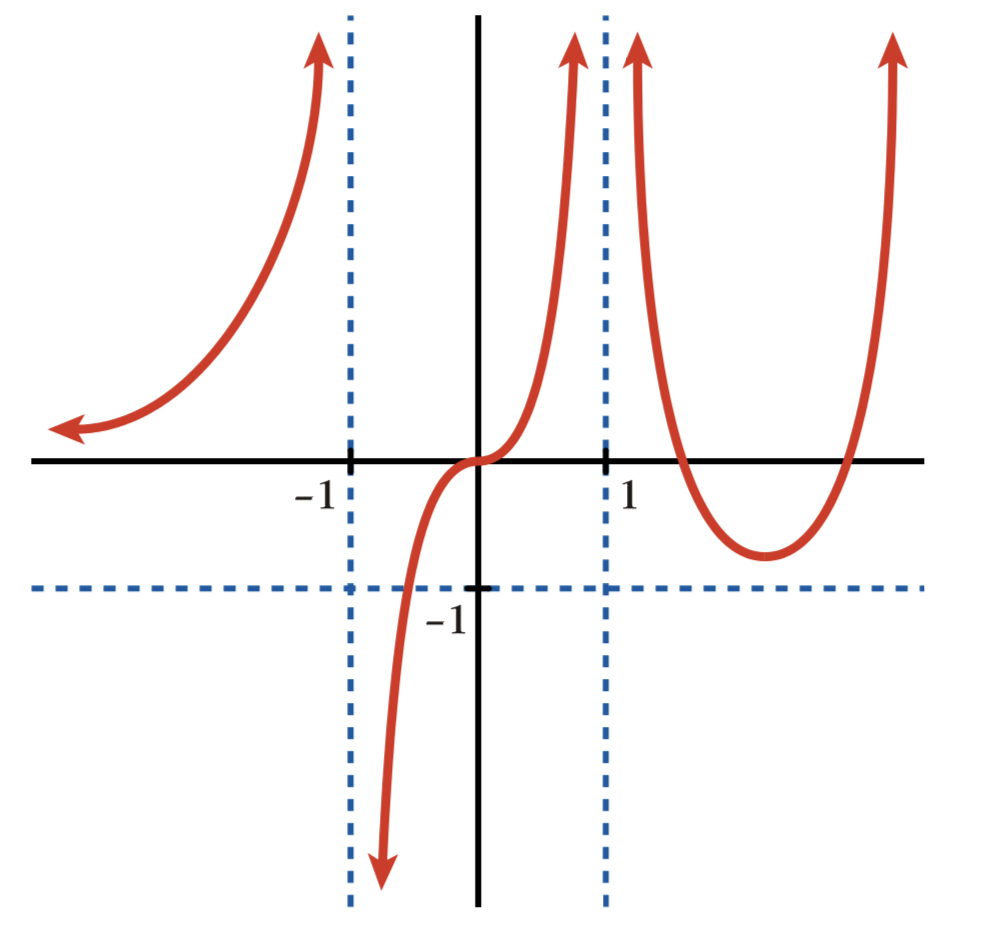
\includegraphics[width=5.2cm]{grafica1.jpg}
  \task $g(x)$:\par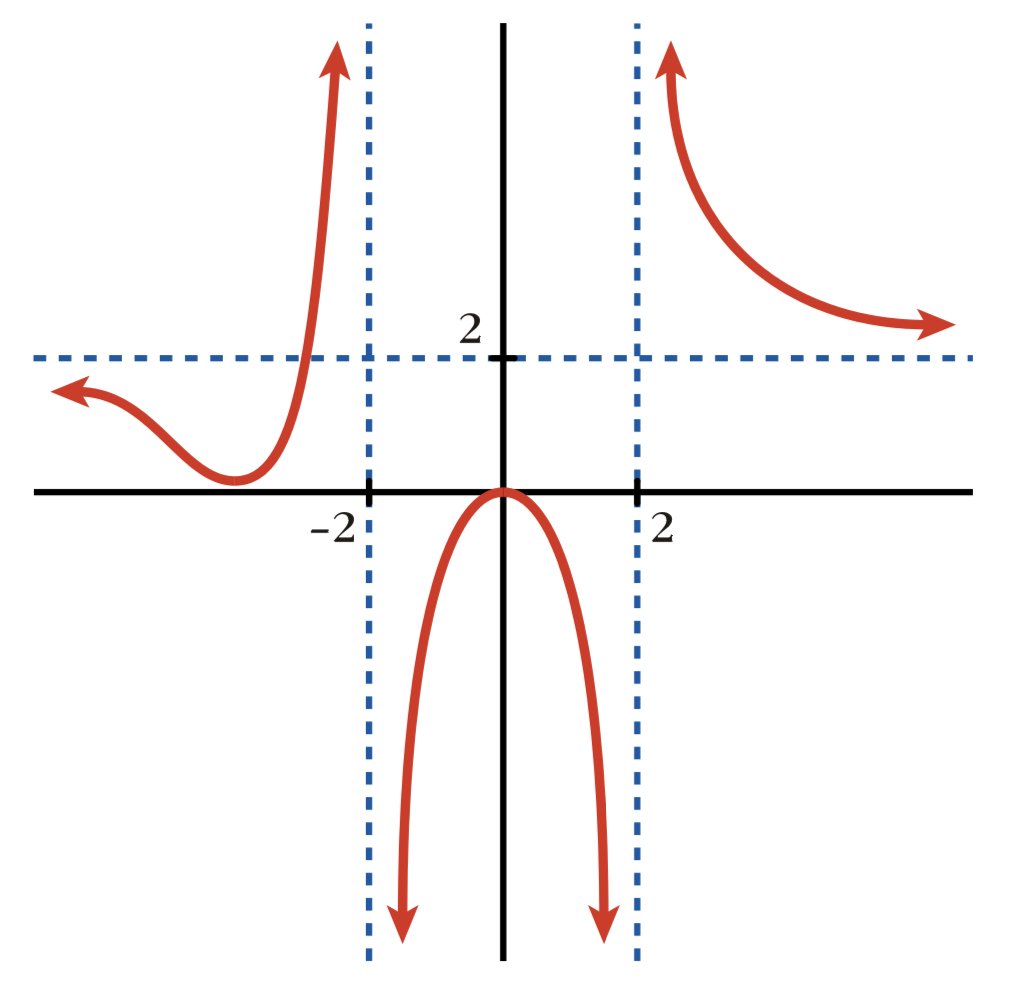
\includegraphics[width=5.2cm]{grafica2.jpg}
\end{tasks}\recorda{Per a $x\to+\infty$ mira el \textbf{final dret} de la gràfica; per a $x\to-\infty$, el \textbf{final esquerre}. Les rectes discontínues són asímptotes.}

\ex{2} Llig a cada gràfica el límit quan $x\to+\infty$ i quan $x\to-\infty$. Fixa't bé en el domini de cada funció:\begin{tasks}(3)
  \task \begin{tikzpicture}[scale=0.42,baseline=(current bounding box.center)]\begin{scope}\draw[muted!30,very thin] (-1,-3) grid (5,2);\draw[-latex,thick] (-1,0)--(5.4,0);\draw[-latex,thick] (0,-3)--(0,2.4);\clip (-1,-3) rectangle (5,2);\draw[accent,line width=1.5pt,smooth,samples=90,domain=0.05:5] plot (\x,{ln(\x)});\node[below,font=\scriptsize] at (1,0) {$1$};\node[left,font=\scriptsize] at (0,1) {$1$};\end{scope}\end{tikzpicture}
  \task \begin{tikzpicture}[scale=0.42,baseline=(current bounding box.center)]\begin{scope}\draw[muted!30,very thin] (-4,-1) grid (5,3);\draw[-latex,thick] (-4,0)--(5.4,0);\draw[-latex,thick] (0,-1)--(0,3.4);\clip (-4,-1) rectangle (5,3);\draw[accent,line width=1.5pt,smooth,samples=90,domain=-3:5] plot (\x,{sqrt(\x+3)});\fill[accent] (-3,0) circle (0.17);\node[below,font=\scriptsize] at (-3,0) {$-3$};\node[below,font=\scriptsize] at (1,0) {$1$};\end{scope}\end{tikzpicture}
  \task \begin{tikzpicture}[scale=0.42,baseline=(current bounding box.center)]\begin{scope}\draw[muted!30,very thin] (-3,-1) grid (3,3);\draw[-latex,thick] (-3,0)--(3.4,0);\draw[-latex,thick] (0,-1)--(0,3.4);\clip (-3,-1) rectangle (3,3);\draw[accent,line width=1.5pt] (2,0) arc (0:180:2);\fill[accent] (-2,0) circle (0.17);\fill[accent] (2,0) circle (0.17);\node[below,font=\scriptsize] at (-2,0) {$-2$};\node[below,font=\scriptsize] at (2,0) {$2$};\end{scope}\end{tikzpicture}
\end{tasks}

\ex{1} Calcula els límits següents:\begin{tasks}(4)
  \task $\displaystyle\lim_{x\to +\infty}(3x^4-2x+7)$
  \task $\displaystyle\lim_{x\to -\infty}(-x^3+4x^2)$
  \task $\displaystyle\lim_{x\to -\infty}(2x^5-x^2)$
  \task $\displaystyle\lim_{x\to +\infty}(5-2x^2)$
\end{tasks}\recorda{El límit d'un polinomi quan $x\to\pm\infty$ és el del seu \textbf{terme de major grau}. Compte amb el signe: $(-\infty)^{\text{parell}}=+\infty$ i $(-\infty)^{\text{senar}}=-\infty$.}

\ex{1} Calcula comparant els graus del numerador i del denominador:\begin{tasks}(3)
  \task $\displaystyle\lim_{x\to +\infty}\dfrac{2x^3-x}{5x^3+4}$
  \task $\displaystyle\lim_{x\to +\infty}\dfrac{x^2+1}{x^3-2}$
  \task $\displaystyle\lim_{x\to -\infty}\dfrac{4x^4-x}{3x^2+1}$
  \task $\displaystyle\lim_{x\to -\infty}\dfrac{1-3x^2}{x+2}$
  \task $\displaystyle\lim_{x\to +\infty}\dfrac{7x-2}{3-x}$
  \task $\displaystyle\lim_{x\to +\infty}\dfrac{x^5}{100x^4+1}$
\end{tasks}\recorda{$\displaystyle\lim_{x\to\pm\infty}\frac{P(x)}{Q(x)}=\lim_{x\to\pm\infty}\frac{a_nx^n}{b_mx^m}$: \ si $n>m$, $\pm\infty$; \ si $n=m$, $\frac{a_n}{b_m}$; \ si $n<m$, $0$.}

\ex{2} Calcula els límits següents amb arrels i exponencials:\begin{tasks}(3)
  \task $\displaystyle\lim_{x\to +\infty}\dfrac{\sqrt{9x^2+1}}{2x-5}$
  \task $\displaystyle\lim_{x\to +\infty}\dfrac{\sqrt{x^3+x}}{x+4}$
  \task $\displaystyle\lim_{x\to +\infty}\dfrac{\sqrt[3]{8x^3-1}}{x}$
  \task $\displaystyle\lim_{x\to -\infty}\left(3^x+1\right)$
  \task $\displaystyle\lim_{x\to -\infty}0{,}4^{x}$
  \task $\displaystyle\lim_{x\to +\infty}\left(\tfrac{5}{2}\right)^{-x}$
\end{tasks}

\ex{3} Calcula $\displaystyle\lim_{x\to +\infty}\dfrac{6x+1}{\sqrt{4x^2+3}}$ i $\displaystyle\lim_{x\to -\infty}\dfrac{6x+1}{\sqrt{4x^2+3}}$. Per què no donen el mateix?

\ex{3} \textbf{Repàs.} Calcula els límits següents. Compte amb el signe de $x$ quan $x\to-\infty$ i amb el domini de cada funció:\begin{tasks}(2)
  \task $\displaystyle\lim_{x\to -\infty}\dfrac{\sqrt{x^4+1}}{2x^2-1}$
  \task $\displaystyle\lim_{x\to -\infty}\dfrac{\sqrt{x^2-5x+3}}{3x-2}$
  \task $\displaystyle\lim_{x\to -\infty}\left(\sqrt{x+1}-\sqrt{x+2}\right)$
  \task $\displaystyle\lim_{x\to -\infty}\dfrac{\sqrt{x^3-5x+3}}{x^2-2x}$
\end{tasks}


% =====================================================
\seccio{2}{Comparació d'infinits}

\ex{1} Ordena de menor a major ordre d'infinit (quan $x\to+\infty$): \quad $x^3,\ \ 2^x,\ \ \ln x,\ \ \sqrt{x},\ \ e^x,\ \ x^{10}$.\recorda{Quan $x\to+\infty$: \ logaritmes $\ll$ potències $\ll$ exponencials. Entre potències guanya l'exponent major i entre exponencials, la base major.}

\ex{2} Calcula els límits següents comparant infinits:\begin{tasks}(3)
  \task $\displaystyle\lim_{x\to +\infty}\dfrac{x^3}{e^x}$
  \task $\displaystyle\lim_{x\to +\infty}\dfrac{2^x+x^4}{3\cdot2^x}$
  \task $\displaystyle\lim_{x\to +\infty}\dfrac{\ln x}{x^2}$
  \task $\displaystyle\lim_{x\to +\infty}\left(x^{10}-1{,}5^x\right)$
  \task $\displaystyle\lim_{x\to +\infty}\dfrac{e^x}{x^5+x}$
  \task $\displaystyle\lim_{x\to +\infty}\dfrac{3^x+2^x}{3^x-x^2}$
\end{tasks}


% =====================================================
\seccio{3}{Indeterminacions}

\ex{2} Indeterminació $\infty-\infty$ amb fraccions:\begin{tasks}(3)
  \task $\displaystyle\lim_{x\to +\infty}\left(\dfrac{x^2}{x+1}-x\right)$
  \task $\displaystyle\lim_{x\to +\infty}\left(\dfrac{2x^2+1}{x-1}-2x\right)$
  \task $\displaystyle\lim_{x\to +\infty}\left(\dfrac{x^3}{x^2+1}-\dfrac{x^2}{x+1}\right)$
\end{tasks}\recorda{Si la indeterminació $\infty-\infty$ ve d'una resta de fraccions, \textbf{fem la resta} amb denominador comú i calculem el límit del resultat.}

\ex{2} Indeterminació $\infty-\infty$ amb arrels:\begin{tasks}(2)
  \task $\displaystyle\lim_{x\to +\infty}\left(\sqrt{x^2+8x}-x\right)$
  \task $\displaystyle\lim_{x\to +\infty}\left(\sqrt{4x^2+x}-2x\right)$
  \task $\displaystyle\lim_{x\to +\infty}\left(\sqrt{x^2+3x}-\sqrt{x^2-x}\right)$
  \task $\displaystyle\lim_{x\to +\infty}\left(\sqrt{x^2+1}-3x\right)$
\end{tasks}\recorda{Multipliquem i dividim pel \textbf{conjugat}: $(\sqrt A-B)(\sqrt A+B)=A-B^2$. Abans, comprova si els termes principals es cancel·len: si no ho fan, no cal el conjugat.}

\ex{2} Indeterminació $1^{\infty}$:\begin{tasks}(3)
  \task $\displaystyle\lim_{x\to +\infty}\left(1+\dfrac5x\right)^{x}$
  \task $\displaystyle\lim_{x\to +\infty}\left(\dfrac{x+2}{x-1}\right)^{2x}$
  \task $\displaystyle\lim_{x\to +\infty}\left(\dfrac{2x-1}{2x+3}\right)^{x+1}$
  \task $\displaystyle\lim_{x\to +\infty}\left(\dfrac{x^2+3}{x^2-1}\right)^{x^2}$
  \task $\displaystyle\lim_{x\to +\infty}\left(\dfrac{3x+1}{x+2}\right)^{x}$
  \task $\displaystyle\lim_{x\to -\infty}\left(\dfrac{x-4}{x}\right)^{3x}$
\end{tasks}\recorda{Si $\lim f(x)=1$ i $\lim g(x)=\pm\infty$: \ $\lim f(x)^{g(x)}=e^{\lim\,(f(x)-1)\cdot g(x)}$. Si la base no tendeix a 1, no hi ha indeterminació.}

\ex{2} Indeterminació $\frac{\infty}{\infty}$ amb arrels:\begin{tasks}(2)
  \task $\displaystyle\lim_{x\to +\infty}\dfrac{\sqrt{x^2+5}+3x}{2x-1}$
  \task $\displaystyle\lim_{x\to +\infty}\dfrac{\sqrt{x^4+1}-x}{x^2+3}$
\end{tasks}

\ex{2} \pau{Aragó, EvAU extraordinària 2020} Donada la funció\[f(x)=\begin{cases}\dfrac{3}{x+1}&\text{si }x<-1\\[3pt]x^3-4x^2+2x-10&\text{si }-1\leq x\leq4\\[3pt]\sqrt{4x^2-7x}-2x&\text{si }x>4\end{cases}\]calcula $\displaystyle\lim_{x\to+\infty}f(x)$. (La continuïtat d'aquesta funció es demana a la secció 6.)

\ex{2} \pau{Balears, PBAU extraordinària 2021} El nombre d'individus, en milions, d'una població ve determinat per la funció $P(t)=\dfrac{2+t+t^2}{t^2+2t+1}$, on $t\geq0$ mesura el nombre d'anys transcorreguts.\begin{tasks}(1)
  \task Quina és la població inicial ($t=0$) i la població després de 5 anys?
  \task A partir de quin moment la població serà inferior a un milió d'individus?
  \task Amb el pas dels anys, cap a quin valor tendirà el nombre d'individus de la població?
\end{tasks}

\ex{2} \pau{Castella i Lleó, EBAU juny 2017} El benefici, en milers d'euros, d'una empresa transcorreguts $x$ mesos és\[f(x)=\begin{cases}20x^2-20x+32&\text{si }0<x\leq1\\[3pt]\dfrac{90x-45}{x+8}+27&\text{si }x>1\end{cases}\]Determina el benefici de l'empresa a molt llarg termini.

\ex{3} \pau{Catalunya, PAU setembre 2018} Se sap que la funció $f(x)=\dfrac{ax+b}{cx+1}$ passa pel punt $(2,-5)$ i que les rectes $x=1$ i $y=2$ són, respectivament, la seua asímptota vertical i horitzontal. Calcula $a$, $b$ i $c$.

\ex{2} \textbf{Repàs.} Calcula els límits següents quan $x\to-\infty$. Abans de res, comprova si de veritat hi ha una indeterminació:\begin{tasks}(2)
  \task $\displaystyle\lim_{x\to -\infty}\left(\dfrac{x^2}{x-3}-\dfrac{x^2}{5-x}\right)$
  \task $\displaystyle\lim_{x\to -\infty}\left(\dfrac{3x^2}{x+1}-\dfrac{x^3}{x^2+1}\right)$
  \task $\displaystyle\lim_{x\to -\infty}\left(\sqrt{x^2+x}-\sqrt{x^2+1}\right)$
  \task $\displaystyle\lim_{x\to -\infty}\left(2x-\sqrt{x^2+x}\right)$
\end{tasks}

\ex{2} \textbf{Repàs.} Calcula:\begin{tasks}(3)
  \task $\displaystyle\lim_{x\to -\infty}\left(\dfrac{3x+4}{2x+5}\right)^{x-1}$
  \task $\displaystyle\lim_{x\to -\infty}\left(\dfrac{2x+1}{2x-1}\right)^{x-1}$
  \task $\displaystyle\lim_{x\to -\infty}\left(\dfrac{x^2+1}{x^2-1}\right)^{\frac{x^2-4}{x-1}}$
\end{tasks}


% =====================================================
\seccio{4}{Límits en un punt i indeterminació 0/0}

\ex{1} Torna a les gràfiques de $f$ i $g$ de l'exercici \ref{ex:g1} i calcula els límits següents, estudiant els límits laterals quan calga:\begin{tasks}(3)
  \task $\displaystyle\lim_{x\to -1}f(x)$
  \task $\displaystyle\lim_{x\to 1}f(x)$
  \task $\displaystyle\lim_{x\to 0}f(x)$
  \task $\displaystyle\lim_{x\to -2}g(x)$
  \task $\displaystyle\lim_{x\to 2}g(x)$
  \task $\displaystyle\lim_{x\to 0}g(x)$
\end{tasks}

\ex{1} \label{ex:g4}Donada la gràfica de la funció $f(x)$, calcula $\displaystyle\lim_{x\to+\infty}f(x)$, $\displaystyle\lim_{x\to-\infty}f(x)$ i $\displaystyle\lim_{x\to0}f(x)$.\par\smallskip{\centering \begin{tikzpicture}[scale=0.5,baseline=(current bounding box.center)]\begin{scope}\draw[muted!30,very thin] (-4,-3) grid (4,4);\draw[-latex,thick] (-4,0)--(4.4,0);\draw[-latex,thick] (0,-3)--(0,4.4);\clip (-4,-3) rectangle (4,4);\draw[accent,line width=1.5pt,smooth,samples=90,domain=-3.46:0] plot (\x,{\x*\x/2-2});\draw[accent,line width=1.5pt,smooth,samples=90,domain=0:4] plot (\x,{1+1/(\x+1)});\draw[teal,dashed] (-4,1)--(4,1);\filldraw[fill=white,draw=accent,line width=1.1pt] (0,-2) circle (0.17);\fill[accent] (0,2) circle (0.17);\node[below,font=\scriptsize] at (1,0) {$1$};\node[left,font=\scriptsize] at (0,1) {$1$};\end{scope}\end{tikzpicture}\par}

\ex{1} Calcula els límits següents. Quan siga necessari, estudia els límits laterals:\begin{tasks}(3)
  \task $\displaystyle\lim_{x\to 2}(x^3-2x+1)$
  \task $\displaystyle\lim_{x\to -1}\dfrac{x^2+3}{x-1}$
  \task $\displaystyle\lim_{x\to 3}\dfrac{2x}{x-3}$
  \task $\displaystyle\lim_{x\to 0}\dfrac{x-1}{x^2}$
  \task $\displaystyle\lim_{x\to 4^+}\sqrt{x-4}$
  \task $\displaystyle\lim_{x\to 1}\dfrac{x+1}{(x-1)^3}$
\end{tasks}\recorda{Si en substituir ix $\frac{k}{0}$ amb $k\neq0$, el límit és infinit: estudiem el signe per l'esquerra i per la dreta.}

\ex{2} Calcula $\displaystyle\lim_{x\to2}f(x)$ i $\displaystyle\lim_{x\to-1}f(x)$, si existeixen, per a\[f(x)=\begin{cases}x^2-3&\text{si }x<-1\\[3pt]2x&\text{si }-1\leq x<2\\[3pt]\dfrac{8}{x}&\text{si }x\geq2\end{cases}\]

\ex{2} Resol les indeterminacions $\frac00$ factoritzant:\begin{tasks}(3)
  \task $\displaystyle\lim_{x\to 3}\dfrac{x^2-5x+6}{x^2-9}$
  \task $\displaystyle\lim_{x\to 2}\dfrac{x^3-8}{x-2}$
  \task $\displaystyle\lim_{x\to 1}\dfrac{x^3-x^2-x+1}{x^2-1}$
  \task $\displaystyle\lim_{x\to 1}\dfrac{x^4-1}{x^2-x}$
  \task $\displaystyle\lim_{x\to -3}\dfrac{x^2+3x}{x^2+6x+9}$
  \task $\displaystyle\lim_{x\to 4}\dfrac{\sqrt{x+5}-3}{x-4}$
\end{tasks}\recorda{Si $P(a)=Q(a)=0$, tots dos són divisibles per $(x-a)$: factoritzem (Ruffini, identitats notables, factor comú), simplifiquem i tornem a substituir.}

\ex{2} \textbf{Repàs.} Calcula els límits següents:\begin{tasks}(3)
  \task $\displaystyle\lim_{x\to 3}\dfrac{x-3}{x^3-5x^2+3x+9}$
  \task $\displaystyle\lim_{x\to 2}\left(\dfrac{2}{x-2}-\dfrac{x+1}{x^2-2x}\right)$
  \task $\displaystyle\lim_{x\to 2}\dfrac{x^2+x-6}{x^2-x-1}$
  \task $\displaystyle\lim_{x\to 2}\left(\dfrac{x+2}{2x}\right)^{\frac{x^2-4}{x-1}}$
  \task $\displaystyle\lim_{x\to -1}\dfrac{x^3-2x^2+2x+5}{x^2-6x-7}$
  \task $\displaystyle\lim_{x\to 2}\dfrac{2x^2+x-10}{x^3-3x^2+4}$
\end{tasks}


% =====================================================
\seccio{5}{Continuïtat en un punt. Funcions racionals}

\ex{1} Torna a la gràfica de $f$ de l'exercici \ref{ex:g1}. Existeix $\displaystyle\lim_{x\to1}f(x)$? Per què la funció no és contínua en $x=1$? I la funció de l'exercici \ref{ex:g4}, és contínua en $x=0$? Justifica les respostes.

\ex{1} Estudia la continuïtat de cada funció en el punt indicat i, si és discontínua, digues de quin tipus és:\begin{tasks}(2)
  \task $f(x)=\dfrac{x^2-4}{x+2}$ \ en $x=-2$
  \task $g(x)=\dfrac{3}{x-4}$ \ en $x=4$
  \task $h(x)=\begin{cases}x^2+1&\text{si }x<0\\x+1&\text{si }x\geq0\end{cases}$ \ en $x=0$
  \task $k(x)=\begin{cases}2x&\text{si }x\leq1\\x^2+3&\text{si }x>1\end{cases}$ \ en $x=1$
\end{tasks}\recorda{$f$ és contínua en $a$ si: \ 1) $\exists f(a)$; \ 2) $\exists\lim_{x\to a}f(x)$; \ 3) $\lim_{x\to a}f(x)=f(a)$. Tipus: evitable, de salt finit, de salt infinit i asimptòtica.}

\ex{2} Estudia la continuïtat de $f(x)=\dfrac{x^2+x-2}{x^2-4x+3}$ i classifica'n les discontinuïtats.

\ex{2} \pau{Cantàbria, EBAU juliol 2019} Siga la funció $f(x)=\dfrac{x^2-x-12}{x^2-2x-15}$. En quins punts és discontínua? Es pot definir de nou aquesta funció per a evitar alguna discontinuïtat?

\ex{2} \pau{Cantàbria, EBAU ordinària 2020} Donada la funció $f(x)=\dfrac{2x+4}{x^2+5x+6}$:\begin{tasks}(1)
  \task En quins punts és discontínua?
  \task Es pot definir de nou la funció per a evitar alguna discontinuïtat?
  \task Calcula els dos límits laterals en $x=-3$ i interpreta gràficament què passa al voltant d'aquest valor.
\end{tasks}

\ex{2} \pau{Navarra, EvAU ordinària 2021} Estudia la continuïtat de la funció $f(x)=\dfrac{x^2+4x+3}{2x-2}$ i, si escau, indica el tipus de discontinuïtat.


% =====================================================
\seccio{6}{Continuïtat de funcions a trossos}

\ex{1} \pau{Navarra, EvAU extraordinària 2021} Estudia la continuïtat de la funció\[f(x)=\begin{cases}x^2-2x&\text{si }x\leq2\\[3pt]-x^2+6x-8&\text{si }x>2\end{cases}\]\recorda{Primer estudiem la continuïtat de cada tros per separat i després mirem els punts on la funció es trenca: $f(a)$, $\lim_{x\to a^-}f$ i $\lim_{x\to a^+}f$.}

\ex{2} \pau{Castella i Lleó, EBAU setembre 2017} Estudia raonadament la continuïtat de\[f(x)=\begin{cases}\dfrac{1}{4-x^2}&\text{si }0<x<2\\[3pt]2x&\text{si }2\leq x<4\end{cases}\]

\ex{2} \pau{Madrid, EvAU juny 2018} Estudia si és contínua en $x=2$ la funció\[f(x)=\begin{cases}\dfrac{x+2}{x-1}&\text{si }x\leq2\\[3pt]\dfrac{3x^2-2x}{x+2}&\text{si }x>2\end{cases}\]Estudia'n també la continuïtat en tot $\mathbb R$.

\ex{2} \pau{Madrid, EvAU juliol 2018} Determina el domini de $f$ i estudia'n la continuïtat:\[f(x)=\begin{cases}x^3+2e^x&\text{si }x<0\\[3pt]\dfrac{2}{3+x}&\text{si }x\geq0\end{cases}\]

\ex{2} \pau{Aragó, EvAU extraordinària 2020} Estudia la continuïtat de\[f(x)=\begin{cases}\dfrac{3}{x+1}&\text{si }x<-1\\[3pt]x^3-4x^2+2x-10&\text{si }-1\leq x\leq4\\[3pt]\sqrt{4x^2-7x}-2x&\text{si }x>4\end{cases}\]

\ex{3} \pau{Madrid, EvAU juny 2019} Analitza la continuïtat de la funció en tot el seu domini segons els valors de $k$:\[f(x)=\begin{cases}e^x+k&\text{si }x\leq0\\[3pt]1-x^2&\text{si }0<x\leq3\\[3pt]\dfrac{1}{x-3}&\text{si }x>3\end{cases}\]

\ex{2} \textbf{Repàs.} Estudia la continuïtat de les funcions següents en el seu domini:\begin{tasks}(2)
  \task $f(x)=\begin{cases}1&\text{si }x<0\\[3pt]x+1&\text{si }0<x<1\\[3pt]x^2-2x&\text{si }1\leq x\end{cases}$
  \task $g(x)=\begin{cases}3x-x^2&\text{si }x\leq3\\[3pt]x-3&\text{si }3<x<6\\[3pt]0&\text{si }x\geq6\end{cases}$
\end{tasks}


% =====================================================
\seccio{7}{Funcions a trossos amb paràmetres}

\ex{1} \pau{Madrid, EvAU setembre 2017} Calcula el valor del paràmetre real $a$ perquè $f$ siga contínua en tot el seu domini:\[f(x)=\begin{cases}ax+1&\text{si }x<-1\\[3pt]x^2+x-2&\text{si }x\geq-1\end{cases}\]\recorda{Igualem els límits laterals (i $f(a)$) en cada punt on canvia l'expressió. Amb dos paràmetres, obtenim un sistema.}

\ex{1} \pau{Andalusia, PEvAU juny 2019} Determina el valor del paràmetre $a$ perquè $f$ siga contínua en tot el seu domini:\[f(x)=\begin{cases}\dfrac{1}{x-1}&\text{si }x<0\\[3pt]x^2+a&\text{si }x\geq0\end{cases}\]

\ex{2} \pau{Castella-la Manxa, EvAU extraordinària 2020} Per a quin valor de $t$ és contínua en $x=0$ la funció\[f(x)=\begin{cases}x-t&\text{si }x\leq0\\[3pt](x-t)^2-5(x+t)+4&\text{si }x>0\end{cases}\]

\ex{2} \pau{Castella-la Manxa, EvAU extraordinària 2020} Es considera la funció \[f(x)=\begin{cases}-4x+4&\text{si }x\leq c\\[3pt]x^2-4x&\text{si }x>c\end{cases}\]Per a quins valors de $c$ és contínua en $x=c$?

\ex{2} \pau{Balears, PBAU extraordinària 2021} Calculau els valors de $a$ perquè $f(x)$ sigui contínua:\[f(x)=\begin{cases}-4x+a&\text{si }x\leq-2\\[3pt]x^2-5&\text{si }-2<x<1\\[3pt]-7x+3&\text{si }x\geq1\end{cases}\]

\ex{2} \pau{Catalunya, PAU setembre 2018} Trobeu el valor de $a$ i $b$ perquè la funció sigui contínua per a tots els nombres reals:\[f(x)=\begin{cases}2x+3&\text{si }x\leq-1\\[3pt]ax+b&\text{si }-1<x<2\\[3pt]x^2&\text{si }x\geq2\end{cases}\]

\ex{3} \pau{Aragó, EvAU setembre 2018} Calcula $a$ i $b$ sabent que $f$ és contínua en tots els punts:\[f(x)=\begin{cases}ax+1&\text{si }x<-2\\[3pt]\dfrac{x+b}{x^2+1}&\text{si }-2\leq x<0\\[3pt]x^3-9x^2+24x+4&\text{si }x\geq0\end{cases}\]

\ex{3} \pau{Cantàbria, EBAU ordinària 2020} Determina els valors de $a$ i $b$ per als quals la funció és contínua en $x=-1$ i en $x=3$:\[f(x)=\begin{cases}ax^2+2x-1&\text{si }x\leq-1\\[3pt]x^2-5&\text{si }-1<x\leq3\\[3pt]\dfrac{b+x}{3x-2}&\text{si }x>3\end{cases}\]

\ex{3} \pau{Cantàbria, EBAU juliol 2019} Determina els valors de $a$ i $b$ per als quals la funció és contínua en $x=-2$ i en $x=0$:\[f(x)=\begin{cases}-6x+3&\text{si }-4<x<-2\\[3pt]x^2+ax+5&\text{si }-2\leq x<0\\[3pt]\dfrac{x+15}{x+b}&\text{si }0\leq x<3\end{cases}\]

\ex{2} \textbf{Repàs.} Donada la funció\[f(x)=\begin{cases}-\dfrac{1}{x^2}&\text{si }x<1\\[3pt]x^2+ax&\text{si }x\geq1\end{cases}\]\begin{tasks}(1)
  \task Calcula el valor de $a$ perquè la funció siga contínua en $x=1$.
  \task Per al valor de $a$ obtingut, estudia la continuïtat de la funció en el seu domini.
\end{tasks}

\ex{3} \textbf{Repàs.} Calcula els valors dels paràmetres $a$ i $b$ perquè les funcions següents siguen contínues en el seu domini:\begin{tasks}(2)
  \task $f(x)=\begin{cases}\dfrac{1}{x^2}+a&\text{si }x\leq-1\\[3pt]3x^2+4&\text{si }-1<x<1\\[3pt]-x^2+b&\text{si }x\geq1\end{cases}$
  \task $g(x)=\begin{cases}-2x+a&\text{si }x\leq-2\\[3pt]x^2-5&\text{si }-2<x<1\\[3pt]bx+3&\text{si }1\leq x\end{cases}$
\end{tasks}

\vfill
\begin{center}\color{muted}\small\faCheckCircle[regular]\ \ Ànim! Comprova els teus resultats amb la calculadora de límits dels apunts interactius.\end{center}

\end{document}
